% NVIDIA RDSS 2027 - Enterprise Software Test Development Engineer (RDSS Intern)
% Eight-slide English interview presentation, adapted from the original ABC Mapper deck.
% Standalone Beamer source: pdfLaTeX, no external image files required.
% Interview-ready version focused on ABC Mapper and NeoPower.
% NeoPower is a company project: keep discussion high-level and do not imply that
% every current repository module was personally authored during employment.
%
% Slide sequence:
%  1 Cover                 2 Education & Experience   3 Outline
%  4 ABC: Extension       5 ABC: Testing
%  6 NeoPower: Systems    7 NeoPower: Reliability
%  8 Thank You

\documentclass[aspectratio=169,10pt]{beamer}
\usepackage[english]{babel}
\usepackage[utf8]{inputenc}
\usepackage[T1]{fontenc}
\usepackage{lmodern}
\usepackage{amsmath,amssymb}
\usepackage{booktabs}
\usepackage{graphicx}
\usepackage{xcolor}
\usepackage{tikz}
\usetikzlibrary{arrows.meta,positioning,calc,shapes.geometric}
\usepackage{hyperref}
\graphicspath{{./}{figures/}}

% --------- Same Madrid-inspired visual identity as the ABC Mapper deck ---------
\usetheme{Madrid}
\usecolortheme{default}
\definecolor{Ink}{HTML}{243748}
\definecolor{Muted}{HTML}{667B8B}
\definecolor{Accent}{HTML}{347E74}
\definecolor{AccentBlue}{HTML}{507DAD}
\definecolor{SoftMint}{HTML}{E6F4EE}
\definecolor{SoftBlue}{HTML}{E9F2F9}
\definecolor{SoftLilac}{HTML}{F1EEF8}
\definecolor{Paper}{HTML}{FBFCFE}
\definecolor{Divider}{HTML}{D8E4EB}
\setbeamercolor{background canvas}{bg=Paper}
\setbeamercolor{normal text}{fg=Ink}
\setbeamercolor{structure}{fg=Accent}
\setbeamercolor{frametitle}{fg=Ink,bg=SoftBlue}
\setbeamercolor{title}{fg=Ink}
\setbeamercolor{subtitle}{fg=Muted}
\setbeamercolor{block title}{fg=Ink,bg=SoftBlue}
\setbeamercolor{block body}{fg=Ink,bg=white}
\setbeamercolor{item}{fg=Accent}
\setbeamercolor{footline}{fg=Muted,bg=Paper}
\setbeamercolor{panelblue}{fg=Ink,bg=SoftBlue!60}
\setbeamercolor{panelmint}{fg=Ink,bg=SoftMint!72}
\setbeamercolor{panellilac}{fg=Ink,bg=SoftLilac!76}
\setbeamercolor{panelwhite}{fg=Ink,bg=white}
\setbeamerfont{frametitle}{size=\Large,series=\bfseries}
\setbeamerfont{footline}{size=\tiny}
\setbeamertemplate{headline}{}
\setbeamertemplate{navigation symbols}{}
\setbeamertemplate{blocks}[rounded][shadow=false]
\setbeamertemplate{itemize items}[circle]
\setbeamertemplate{footline}{%
  \leavevmode\hbox{%
    \begin{beamercolorbox}[wd=\paperwidth,ht=.30cm,dp=.16cm,rightskip=.60cm plus 1fil]{footline}%
      \hfill\insertframenumber\,/\,\inserttotalframenumber
    \end{beamercolorbox}}%
}
\setbeamertemplate{frametitle}{%
  \nointerlineskip
  \begin{beamercolorbox}[wd=\paperwidth,ht=.77cm,dp=.18cm,leftskip=.64cm]{frametitle}%
    \usebeamerfont{frametitle}\insertframetitle
  \end{beamercolorbox}%
}

% --------- Same basic components, plus lightweight reusable panels ---------
\newcommand{\smalllabel}[1]{{\scriptsize\bfseries\color{Accent}\MakeUppercase{#1}}}
\newcommand{\takeaway}[1]{%
  \begin{beamercolorbox}[rounded=true,sep=0.15cm,wd=\linewidth]{block title}%
    \strut\textbf{#1}\strut
  \end{beamercolorbox}%
}
\newcommand{\minibadge}[2]{%
  \tikz[baseline=(badge.base)]\node[fill=#1,rounded corners=3pt,
    inner xsep=6pt,inner ysep=3pt] (badge) {\scriptsize\bfseries #2};%
}
\newcommand{\softpanel}[3]{%
  \begin{beamercolorbox}[rounded=true,sep=0.16cm,wd=\linewidth]{#1}%
    {\small\bfseries\color{Accent}#2}\par\vspace{0.08cm}
    {\small\color{Ink}#3}%
  \end{beamercolorbox}%
}
\newcommand{\smallpanel}[3]{%
  \begin{beamercolorbox}[rounded=true,sep=0.13cm,wd=\linewidth]{#1}%
    {\small\bfseries\color{Accent}#2}\par\vspace{0.06cm}
    {\scriptsize\color{Ink}#3}%
  \end{beamercolorbox}%
}
\newcommand{\outlinecard}[4]{%
  \begin{beamercolorbox}[rounded=true,sep=0.17cm,wd=\linewidth]{#1}%
    \begin{minipage}[c]{0.34\linewidth}
      {\normalsize\bfseries #2}\par\vspace{0.03cm}
      {\scriptsize\color{Accent}#3}
    \end{minipage}\hfill%
    \begin{minipage}[c]{0.63\linewidth}
      {\small #4}
    \end{minipage}%
  \end{beamercolorbox}%
}
\newcommand{\gate}[3]{%
  \begin{beamercolorbox}[rounded=true,sep=0.15cm,wd=\linewidth]{panelwhite}%
    {\small\bfseries\color{Accent}#1\quad #2}\par\vspace{0.07cm}
    {\scriptsize\color{Muted}#3}%
  \end{beamercolorbox}%
}

\title[Software Development and Testing]{Software Development, Testing \& Reliability}
\subtitle{ABC Mapper / NeoPower System}
\author{Yu-Jui Liang}
\institute{National Taiwan University \quad | \quad Data Science Master's Degree Program}
\date{October 20, 2026}

\begin{document}

% ============================================================
% SLIDE 1 - Cover (same composition as original ABC deck)
% ============================================================
{\setbeamertemplate{footline}{}
\begin{frame}[plain]
  \vspace*{1.00cm}
  \smalllabel{Enterprise Software Test Development Engineer (RDSS Intern)}\par
  \vspace{0.62cm}
  {\raggedright\fontsize{17}{21}\selectfont\bfseries\color{Ink}
    \mbox{Software Development, Testing \& Reliability}\par}
  \vspace{0.43cm}
  {\color{Muted}\normalsize ABC Mapper \quad / \quad NeoPower System\par}
  \vspace{0.94cm}
  {\bfseries Yu-Jui Liang}\par
  \vspace{0.08cm}
  {\normalsize\color{Muted}Data Science Master's Degree Program\par}
  \vspace{0.05cm}
  {\small\color{Muted}National Taiwan University \quad | \quad 20 Oct 2026\par}
  \vfill
  {\color{Accent}\rule{\textwidth}{0.7pt}}\par\vspace{0.03cm}
  {\small\bfseries\color{Muted}Software Development \quad / \quad Verification \& Testing \quad / \quad Debugging}
\end{frame}}

% ============================================================
% SLIDE 2 - Education & Professional Experience
% ============================================================
\begin{frame}{Education \& Professional Experience}
  \vspace{0.05cm}
  \smalllabel{01 / Background}\par
  \vspace{0.22cm}

  \begin{columns}[T,onlytextwidth]

    % ----- Education -----
    \begin{column}{0.49\textwidth}
      \begin{beamercolorbox}[
        rounded=true,sep=0.20cm,wd=\linewidth
      ]{panelblue}

        {\normalsize\bfseries\color{AccentBlue}
          Education}\par
        \vspace{0.24cm}

        {\small\bfseries
          National Taiwan University}\par
        \vspace{0.06cm}
        {\small
          M.S. Candidate, Data Science
          Master's Degree Program}\par
        \vspace{0.05cm}
        {\scriptsize\color{Muted}
          Expected Graduation: June 2027}\par

        \vspace{0.26cm}
        {\color{Divider}\rule{0.92\linewidth}{0.4pt}}
        \vspace{0.19cm}

        {\small\bfseries
          National Chengchi University}\par
        \vspace{0.06cm}
        {\small
          B.S. in Computer Science}\par
        {\small
          Double Major in Electronic Physics}\par
        \vspace{0.05cm}
        {\scriptsize\color{Muted}
          Sep. 2021 -- Jun. 2025}\par

      \end{beamercolorbox}
    \end{column}

    % ----- Professional Experience -----
    \begin{column}{0.49\textwidth}
      \begin{beamercolorbox}[
        rounded=true,sep=0.20cm,wd=\linewidth
      ]{panelmint}

        {\normalsize\bfseries\color{Accent}
          Professional Experience}\par
        \vspace{0.24cm}

        {\small\bfseries
          AIMobile Co., Ltd.}\par
        {\scriptsize\color{Muted}
          Inventec Group}\par
        \vspace{0.06cm}
        {\small
          Contract Software Engineer}\par
        \vspace{0.05cm}
        {\scriptsize\color{Muted}
          Apr. 2025 -- Jul. 2025}\par

        \vspace{0.26cm}
        {\color{Divider}\rule{0.92\linewidth}{0.4pt}}
        \vspace{0.19cm}

        {\small\bfseries
          Neopower Technologies\\Co., Ltd.}\par
        \vspace{0.06cm}
        {\small
          Contract Software Engineer}\par
        \vspace{0.05cm}
        {\scriptsize\color{Muted}
          Jun. 2023 -- Mar. 2025}\par

      \end{beamercolorbox}
    \end{column}

  \end{columns}
\end{frame}


% ============================================================
% SLIDE 3 - Outline / two projects
% ============================================================
\begin{frame}{Outline}
  \vspace{0.04cm}
  \smalllabel{02 / Presentation Overview}\par
  \vspace{0.09cm}
  \takeaway{Two projects, two complementary software engineering experiences.}
  \vspace{0.25cm}
  \outlinecard{panelblue}{01 \quad ABC Mapper}{Software Extension \& Integration}{%
    Modular C++ development, backward compatibility, and regression testing.}
  \vspace{0.17cm}
  \outlinecard{panelmint}{02 \quad NeoPower}{Backend Development \& Maintenance}{%
    API integration, system operations, simulation, and debugging in a smart charging platform.}

  \vfill
  {\scriptsize\color{Muted}Focus: engineering decisions, verification strategies, and lessons from implementation.}
\end{frame}



% ============================================================
% SLIDE 4 - ABC Mapper: Extension and integration
% ============================================================
\begin{frame}{ABC Mapper: Software Extension \& Integration}
  \vspace{0.01cm}
  \smalllabel{03 / ABC Mapper -- 1 of 2}\par\vspace{0.09cm}
  \takeaway{Extend an existing EDA tool while preserving its original single-output flow.}
  \vspace{0.06cm}
  \minibadge{SoftBlue}{Architecture: Add a Parallel MO Path}\par
  \vspace{0.02cm}
  \begin{center}
  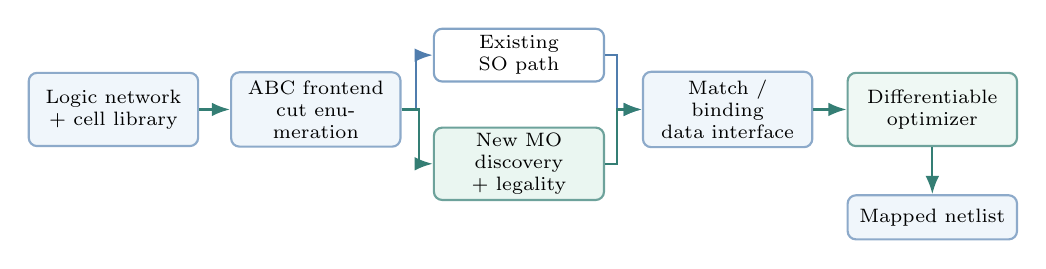
\begin{tikzpicture}[>=Latex,font=\scriptsize,line width=.78pt]
    \tikzset{
      corebox/.style={draw=AccentBlue!65,fill=SoftBlue!70,rounded corners=3pt,
        text width=1.94cm,minimum height=.93cm,align=center,inner sep=3pt},
      sobox/.style={draw=AccentBlue!70,fill=white,rounded corners=3pt,
        text width=2.02cm,minimum height=.67cm,align=center,inner sep=2pt},
      mobox/.style={draw=Accent!72,fill=SoftMint!85,rounded corners=3pt,
        text width=2.02cm,minimum height=.67cm,align=center,inner sep=2pt}
    }
    \node[corebox] (src) at (0,0) {Logic network\\+ cell library};
    \node[corebox] (abc) at (2.57,0) {ABC frontend\\cut enumeration};
    \node[sobox] (so) at (5.15,.69) {Existing SO path};
    \node[mobox] (mo) at (5.15,-.69) {New MO discovery\\+ legality};
    \node[corebox] (iface) at (7.80,0) {Match / binding\\data interface};
    \node[corebox,fill=SoftMint!65,draw=Accent!72] (opt) at (10.40,0)
        {Differentiable\\optimizer};
    \node[corebox,minimum height=.56cm] (out) at (10.40,-1.37) {Mapped netlist};
    \draw[->,Accent,thick] (src.east)--(abc.west);
    \draw[->,AccentBlue,thick] (abc.east)--++(.18,0)|-(so.west);
    \draw[->,Accent,thick] (abc.east)--++(.22,0)|-(mo.west);
    \draw[->,AccentBlue,thick] (so.east)--++(.15,0)|-(iface.west);
    \draw[->,Accent,thick] (mo.east)--++(.15,0)|-(iface.west);
    \draw[->,Accent,thick] (iface.east)--(opt.west);
    \draw[->,Accent,thick] (opt.south)--(out.north);
  \end{tikzpicture}
  \end{center}
  \vspace{0.02cm}
  \begin{columns}[T,onlytextwidth]
    \begin{column}{0.486\textwidth}
      \smallpanel{panelblue}{Non-invasive Software Extension}{%
        Independent MO candidate discovery and output-pair binding; legacy SO workflow kept separate.}
    \end{column}
    \begin{column}{0.486\textwidth}
      \smallpanel{panelmint}{Modular Toolchain Integration}{%
        ABC match export $\rightarrow$ differentiable SO/MO selection $\rightarrow$ netlist reconstruction.}
    \end{column}
  \end{columns}
  % The MO differentiable-optimization path is experimental; the legacy SO path remains separate.
\end{frame}

% ============================================================
% SLIDE 5 - ABC Mapper: testing strategy
% ============================================================
\begin{frame}{ABC Mapper: Correctness \& Regression Testing}
  \vspace{0.02cm}
  \smalllabel{04 / ABC Mapper -- 2 of 2}\par\vspace{0.09cm}
  \takeaway{New mapping features must preserve the original Boolean behavior.}
  \vspace{0.23cm}
  \begin{columns}[T,onlytextwidth]
    \begin{column}{0.315\textwidth}
      \smallpanel{panelblue}{01 \quad Compatibility}{%
        SO-only smoke / regression cases verify that the pre-existing flow is not disrupted.}
    \end{column}
    \begin{column}{0.315\textwidth}
      \smallpanel{panelmint}{02 \quad Candidate Legality}{%
        Check MO output roles, pin compatibility, pair structure, and match-data consistency.}
    \end{column}
    \begin{column}{0.315\textwidth}
      \smallpanel{panellilac}{03 \quad End-to-End CEC}{%
        Compare original network behavior against the generated mapped netlist.}
    \end{column}
  \end{columns}
  \vspace{0.13cm}
  \minibadge{SoftBlue}{Implementation-to-Verification Loop}\par
  \vspace{0.15cm}
  \begin{center}
  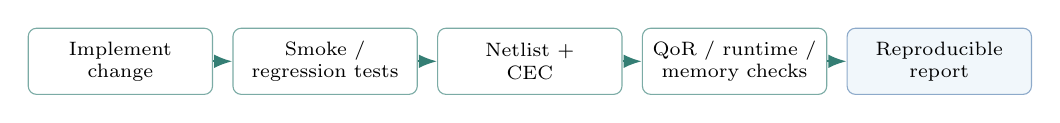
\begin{tikzpicture}[>=Latex,font=\scriptsize]
    \tikzset{check/.style={draw=Accent!65,fill=white,rounded corners=3pt,
       minimum height=.84cm,text width=2.13cm,align=center,inner sep=3pt}}
    \node[check] (a) at (0,0) {Implement\\change};
    \node[check] (b) at (2.60,0) {Smoke /\\regression tests};
    \node[check] (c) at (5.20,0) {Netlist +\\CEC};
    \node[check] (d) at (7.80,0) {QoR / runtime /\\memory checks};
    \node[check,draw=AccentBlue!65,fill=SoftBlue!65] (e) at (10.40,0)
      {Reproducible\\report};
    \foreach \u/\v in {a/b,b/c,c/d,d/e}{\draw[->,thick,Accent] (\u.east)--(\v.west);}
  \end{tikzpicture}
  \end{center}
  \vspace{0.10cm}
  \begin{beamercolorbox}[rounded=true,sep=.16cm,wd=\linewidth]{panelmint}
    {\small\bfseries\color{Ink}Validation principle:}\quad
    {\small CEC proves functional equivalence; area / delay optimization is evaluated separately.}
  \end{beamercolorbox}
\end{frame}

% ============================================================
% SLIDE 6 - NeoPower: architecture
% ============================================================
\begin{frame}{NeoPower: System Architecture \& Integration}
  \vspace{0.01cm}
  \smalllabel{05 / NeoPower -- 1 of 2}\par\vspace{0.09cm}
    \takeaway{An electric vehicle (EV) charging management platform integrating APIs and backend services.}
  \vspace{0.04cm}
  \minibadge{SoftBlue}{High-Level Service Architecture}\par\vspace{0.00cm}
  \begin{center}
  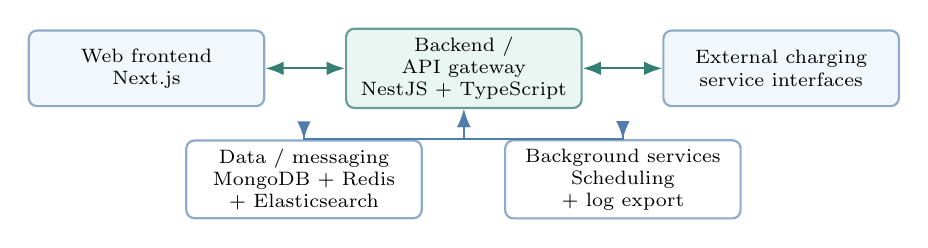
\begin{tikzpicture}[>=Latex,font=\scriptsize,line width=.78pt]
    \tikzset{service/.style={draw=AccentBlue!65,fill=SoftBlue!62,rounded corners=3pt,
      text width=2.78cm,minimum height=.96cm,align=center,inner sep=3pt}}
    \node[service] (ui) at (0,0) {Web frontend\\Next.js};
    \node[service,draw=Accent!75,fill=SoftMint!85] (api) at (4.03,0)
       {Backend / API gateway\\NestJS + TypeScript};
    \node[service] (cpo) at (8.06,0) {External charging\\service interfaces};
    \node[service,fill=white,minimum height=.85cm] (db) at (2.00,-1.41)
       {Data / messaging\\MongoDB + Redis \\ + Elasticsearch};
    \node[service,fill=white,minimum height=.85cm] (jobs) at (6.05,-1.41)
       {Background services\\Scheduling + log export};
    \draw[<->,Accent,thick] (ui.east)--(api.west);
    \draw[<->,Accent,thick] (api.east)--(cpo.west);
    \draw[<->,AccentBlue] (api.south)--++(0,-.38)-|(db.north);
    \draw[<->,AccentBlue] (api.south)--++(0,-.38)-|(jobs.north);
  \end{tikzpicture}
  \end{center}
  \vspace{-0.12cm}
  \begin{columns}[T,onlytextwidth]
    \begin{column}{0.486\textwidth}
      \smallpanel{panelblue}{Backend / API Development}{%
        Service boundaries, request-response contracts, and integrations with charging operations.}
    \end{column}
    \begin{column}{0.486\textwidth}
    \smallpanel{panelmint}{Container-Based Service Isolation}{%
        Isolated individual services in containers to simplify
        deployment, maintenance, and troubleshooting.}
    \end{column}
  \end{columns}
\end{frame}

% ============================================================
% SLIDE 7 - NeoPower: Testing & Reliability Engineering
% ============================================================
\begin{frame}{NeoPower: Testing \& Reliability Engineering}
  \vspace{0.02cm}
  \smalllabel{06 / NeoPower -- 2 of 2}\par\vspace{0.09cm}

  \takeaway{Validate changes through real-world simulation,
  regression testing, and field evaluation.}

  \vspace{0.10cm}
  \begin{columns}[T,onlytextwidth]
    \begin{column}{0.486\textwidth}
      \softpanel{panelblue}{Pre-Deployment Testing}{%
        \textbullet\ External vendor / client simulators\\[1.2mm]
        \textbullet\ Production-derived test scenarios\\[1.2mm]
        \textbullet\ High load and multi-charger failures\\[1.2mm]
        \textbullet\ Scenario-based regression testing}
    \end{column}

    \begin{column}{0.486\textwidth}
    \softpanel{panelmint}{Post-Deployment A/B Testing}{%
        \textbullet\ Compare existing and updated implementations\\[1.2mm]
        \textbullet\ Time-based testing at the same charging site\\[1.2mm]
        \textbullet\ Cross-site comparison under similar conditions\\[1.2mm]
        \textbullet\ Operational metrics and customer feedback}
    \end{column}
  \end{columns}

  % ----- Field-informed testing workflow -----
  \vspace{0.18cm}
  \minibadge{SoftBlue}{Field-Informed Regression Workflow}\par
  \vspace{0.15cm}

  \begin{center}
  
\begin{tikzpicture}[>=Latex,font=\scriptsize]
    \tikzset{
      flowstep/.style={
        draw=Accent!65,
        fill=white,
        rounded corners=3pt,
        minimum height=.87cm,
        text width=2.07cm,
        align=center,
        inner sep=3pt
      }
    }

    \node[flowstep] (a) at (0,0)
      {Collect\\Field Data};

    \node[flowstep] (b) at (2.55,0)
      {Reproduce\\Scenario};

    \node[flowstep] (c) at (5.10,0)
      {Simulate\\Vendor};

    \node[flowstep] (d) at (7.65,0)
      {Run\\Regression};

    \node[flowstep,fill=SoftMint!70] (e) at (10.20,0)
      {Deploy \&\\Monitor};

    \foreach \u/\v in {a/b,b/c,c/d,d/e}{
      \draw[->,thick,Accent] (\u.east)--(\v.west);
    }
  \end{tikzpicture}
  \end{center}

  \vspace{-0.04cm}
  {\small\color{Muted}
    Historical incidents become reusable test scenarios
    for future software releases.
  }

\end{frame}

% ============================================================
% SLIDE 10 - Thank You, matching original ABC deck closing slide
% ============================================================
{\setbeamertemplate{footline}{}
\begin{frame}[plain]
  \vfill
  \begin{center}
    {\fontsize{38}{44}\selectfont\bfseries\color{Ink}Thank You}\par
    \vspace{0.30cm}
    {\Large\color{Accent}Questions \& Discussion}
  \end{center}
  \vfill
\end{frame}}

\end{document}